% !TeX root = vampy.tex
%vampy-notes.tex
% notes for development of VAMPy (image analysis part of VAMP project)
% all figures concerning Phase Contrast images are based on image file
% pshchelo\images\pipettes\PhC\me\micropipettes6\ves_-000100.tif = phc-test1.tif

\section{Development Notes}
\subsection{Extraction of data from images}\label{data}

For now everything is done in Python with different additional packages.

The pseudocode-like draft for the algorithm for processing single image looks like this:
\begin{enumerate}
  \item load picture to array
  \item get user input
  \item calculate positions of pipette walls
  \item calculate pipette radius
  \item calculate the axis of the system
  \item extract data along the axis from the picture
  \item find positions of 3 characteristic points on the axis
  \item calculate all derived parameters (vesicle radius, tip length, surface area, volume)
  \item calculate dilations and tensions and fit them with some defined function
\end{enumerate}

Python packages aside from Python Standard Library used or (probably) going to be used in this program:
\begin{itemize}
	\item \emph{numpy} --- basic package for numeric stuff, defines \emph{array} data type
	\item \emph{scipy} --- depends on \emph{numpy} and provides a lot of mathematical functions, which I most probably will need \cite{scipy}
	\item \emph{wxPython} --- GUI programming
	\item \emph{psyco} --- JIT compiler for Python, may use it to speed up the execution
	\item \emph{Python Image Library (PIL)} --- basic image processing functionality, but may eventually drop it (see Section \ref{loadpic})
	\item \emph{matplotlib} --- for plotting results
\end{itemize}

\subsubsection{Load picture to array}\label{loadpic}

This is done with \emph{scipy} and \emph{PIL}, which allows for direct conversion from image file to \emph{numpy} array.

On the other hand, \emph{wxPython}'s wxImage object could be probably used, thus eliminating the need of \emph{PIL} package, since I'm going to use \emph{wxPython} for GUI programming anyway. Unfortunately, wxImage still doesn't support \emph{numpy}-like array interface as of now, but this is planned feature for addition. Or buffers interface seems to be able to do this \ldots

\subsubsection{Get user input}\label{getinput}

\begin{figure}
	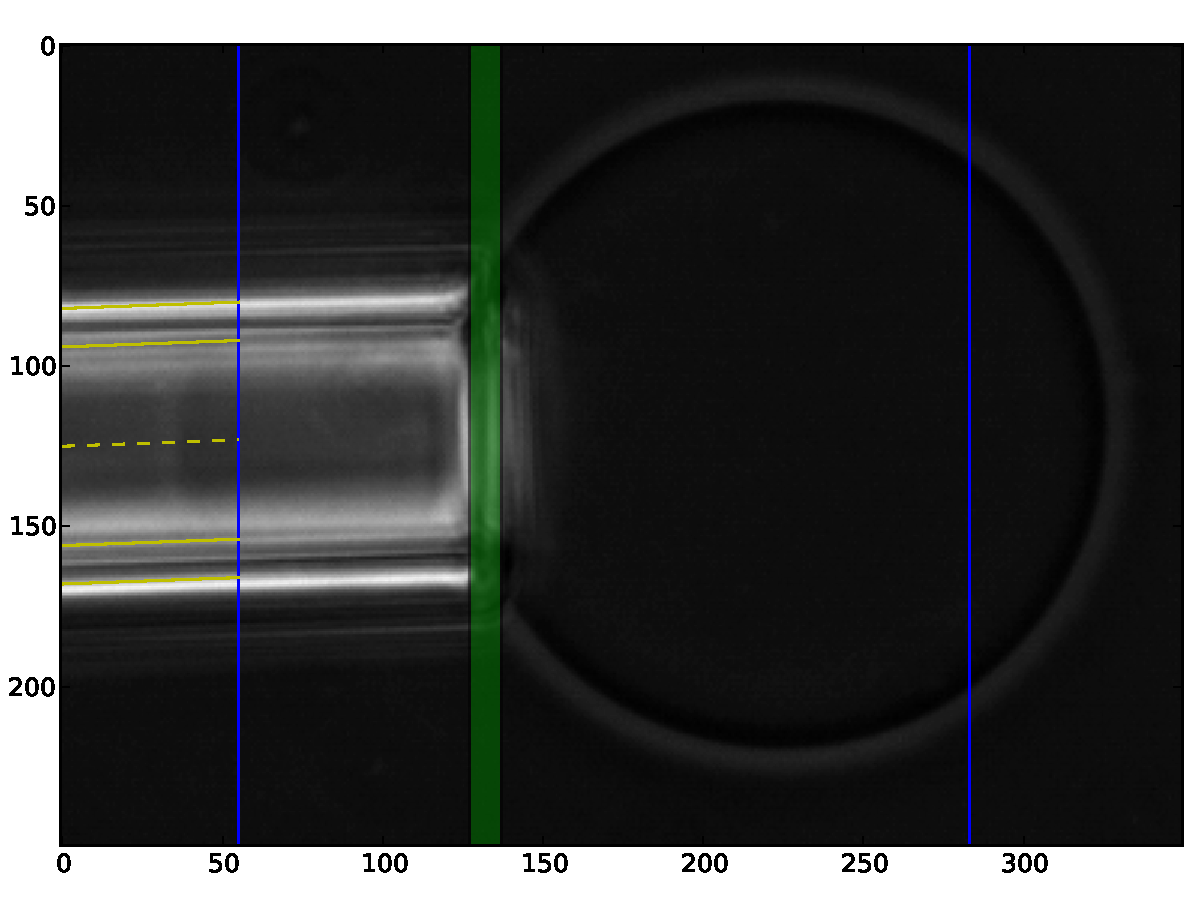
\includegraphics[width=\columnwidth]{figs/userinput.pdf}
	\caption{User supplied parameters visualized on the aspirated vesicle image. Left blue line is $x_{a0}$, right blue line is $x_{v0}$, green region is approximate pipette tip position, yellow lines define the approximate pipette walls positions, yellow dashed line is approximate pipette axis.}
	\label{fig:userinput}
\end{figure}

First of all user should crop the image so that everything but the vesicle is left out and rotate the picture so that the pipette \emph{sticks from left}. Let us assume the size of the image along the x-axis is now $N$. User supplies several sets of coordinates to define approximate regions of features locations (see Figure \ref{fig:userinput}):
\begin{itemize}
	\item overestimated position of the aspirated vesicle part $x_{a0}$ so that the tip of the aspirated vesicle part must be always to the left from this, $ x_a \in (0, x_{a0})$;
	\item overestimated position of the outer part of the vesicle $x_{v0}$ so that the tip of the outer part of the vesicle is always to the right of it, $ x_v \in (x_{v0}, N)$;
	\item approximate position of the pipette tip, $x_{p1}, x_{p2}$ so that the pipette tip is always in this region, $ x_p \in (x_{p1}, x_{p2})$;
	\item approximate positions of pipette walls.
\end{itemize}

\subsubsection{Define pipette walls}\label{pipwalls}
A cross-sections of the pipette are taken in two points $x=0$ and $x=x_{a0}$. The pipette walls are then taken as global minima in the regions corresponding to the approximate pipette walls positions for each cross-section (see Figure \ref{fig:pipcrosssection}), producing sets of coordinates $(x_1,y_1), (x_2,y_2)$ and $(x_3,y_3), (x_4,y_4)$. The $y$-positions can be further defined more accurately with subpixel resolution (see Section~\ref{subpix}).

\begin{figure}%
	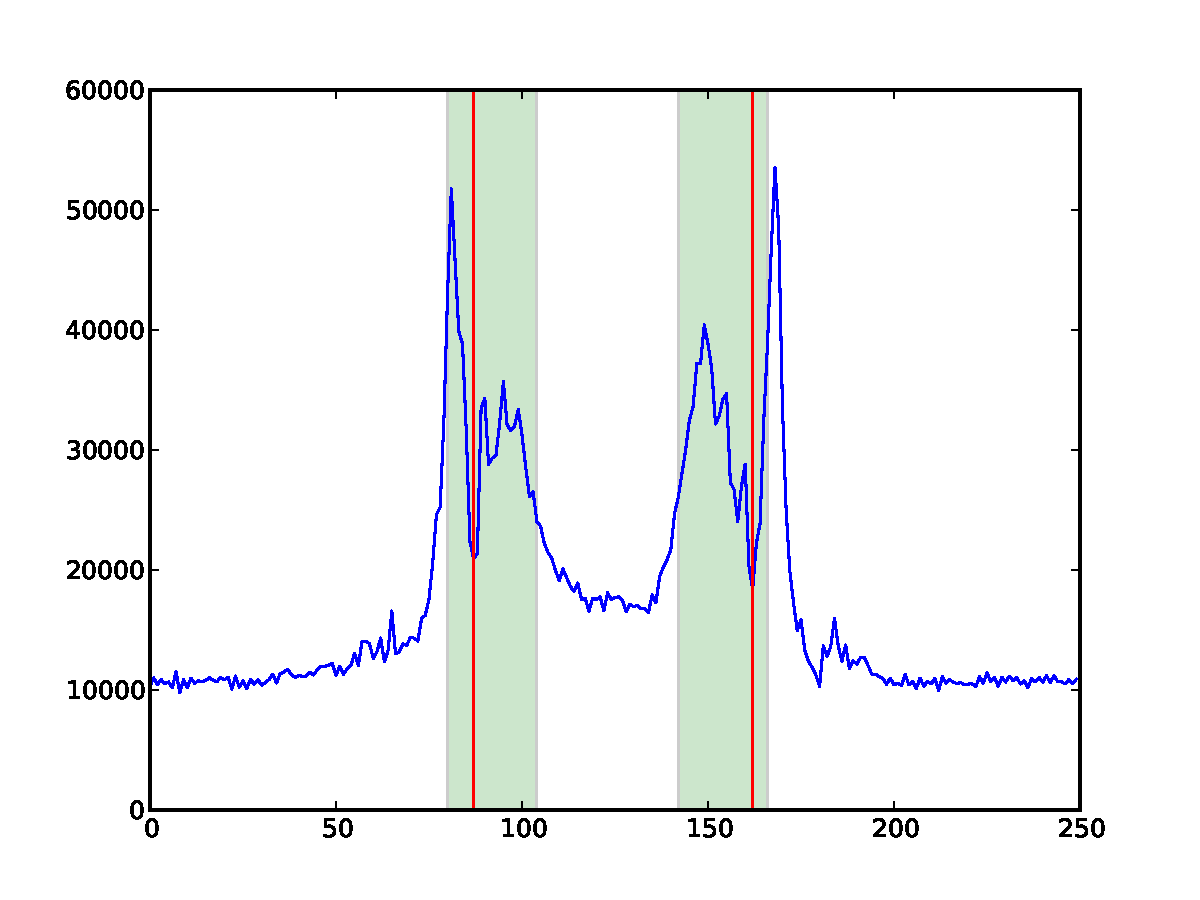
\includegraphics[width=\columnwidth]{figs/pipcrosssection.pdf}%
	\caption{Brightness profile of the pipette cross-section at $x=x_{a0}$. Green regions correspond to user-supplied approximate pipette wall positions, red vertical lines denote the actual found positions of pipette walls.}%
	\label{fig:pipcrosssection}%
\end{figure}

\subsubsection{Calculate pipette radius}\label{calcpiprad}

Distance (unsigned) from point $\left(x_0,y_0\right)$ to line $y=kx+b$ is given by:
\begin{equation}
	\delta = \left|\frac{kx_0+b-y_0}{\sqrt{k^2-1}}\right|\;.
	\label{eq:pointtoline}
\end{equation}
Thus the diameter of the pipette for single image is calculated as mean of distances from every of 4 points to the line corresponding to the opposing wall. Then these values are again averaged between all images.

\subsubsection{Calculate the middle line (axis) of the system}\label{calcaxis}

\begin{figure}
	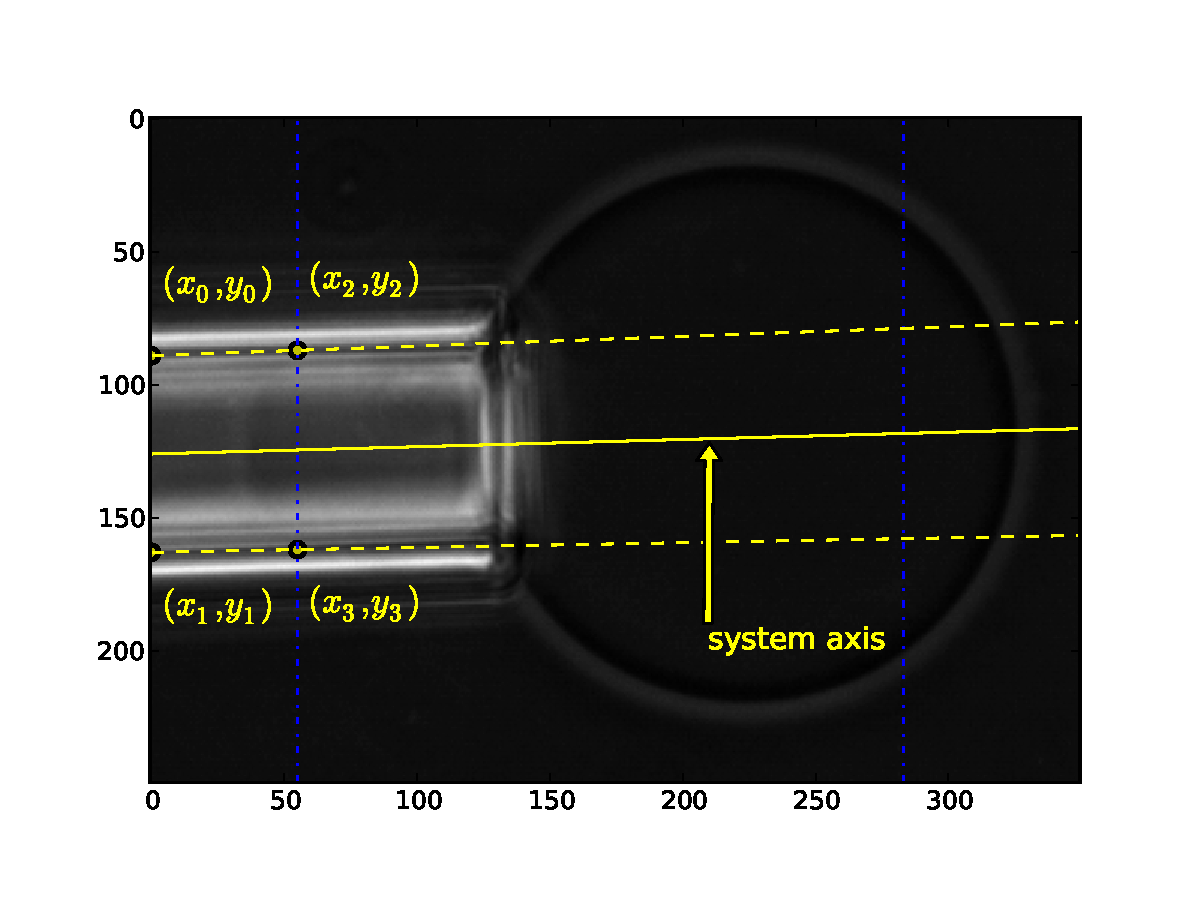
\includegraphics[width=\columnwidth]{figs/pipetteaxis.pdf}
 	\caption{Sketch of general situation of pipette system alignment on the image}
 	\label{fig:pipetteaxis}
\end{figure}

Having obtained the set of reference points from Section~\ref{pipwalls} one builds a system axis as a bisector between straight lines formed by pipette inner walls. This is done by simply defying the line going through 2 middle points $\left(\frac{x_1+x_2}{2}, \frac{y_1+y_2}{2}\right)$ and $\left(\frac{x_3+x_4}{2}, \frac{y_3+y_4}{2}\right)$. Then the axis $y = kx+b$ is defined by coefficients

\begin{equation}
k = \frac{y_1+y_1-y_3-y_4}{x_1+x_2-x_3-x_4}, \; b = \frac{y_1+y_2}{2} - k\frac{x_1+x_2}{2}\;\;.
\label{eq:axis}
\end{equation}

After that the brightness profile along this axis is extracted from image with special function \texttt{scipy.ndimage.map-coordinates}, which returns spline-interpolated values of brightness ``between'' pixels. To define the set of points at which interpolated brightness should be evaluated first intersections of the system axis with boundaries of image are calculated. To define the number of points for evaluation the biggest of differences in $x$ or $y$ coordinates between intersection points is taken.

Small pitfall --- since at the end we need real distances between features, an attention have to be paid to keep the scale of profiles equal. The above procedure does not keep the scale, because the line has only as many points as there are along one of it's coordinates, but it should be $\sqrt{x^2+y^2}$. Hence, the distance between 2 consecutive points on brightness profile along arbitrary tilted straight line with number of evaluated points as defined above corresponds to distance $\epsilon$ in pixels, where
\begin{equation}
\epsilon = \left\{
\begin{array}{ll}
	\sqrt{1+k^2},&\text{if }k < 1\\
	\sqrt{1+\frac{1}{k^2}},&\text{if } k \geq 1 
\end{array}
\right.\;\;,
\label{eq:profilescale}
\end{equation}
so that $1 \leq \epsilon \leq \sqrt{2}$. Thus the procedure of extracting brightness profile must also return the $\epsilon$ value along with profile itself to use it in final steps of determining distances. This is not necessary for profiles used for location of pipette walls, since by design only untilted profiles along pixel lines are used there, thus the scale in preserved.

\subsubsection{Find positions of 3 characteristic points on the axis}\label{points}

We are interested in 3 points on the axis of the system --- intersection of axis with outer vesicle, aspirated tip of a vesicle and the tip of the pipette. These manifest themselves as peaks (positive or negative) or steep jumps on the brightness profile along the axis. What exactly feature corresponds to what point of interest depends on the type of images one analyses.

\begin{itemize}
	\item \textbf{Phase contrast images} \label{phcfeatures}
		
		\begin{figure}
		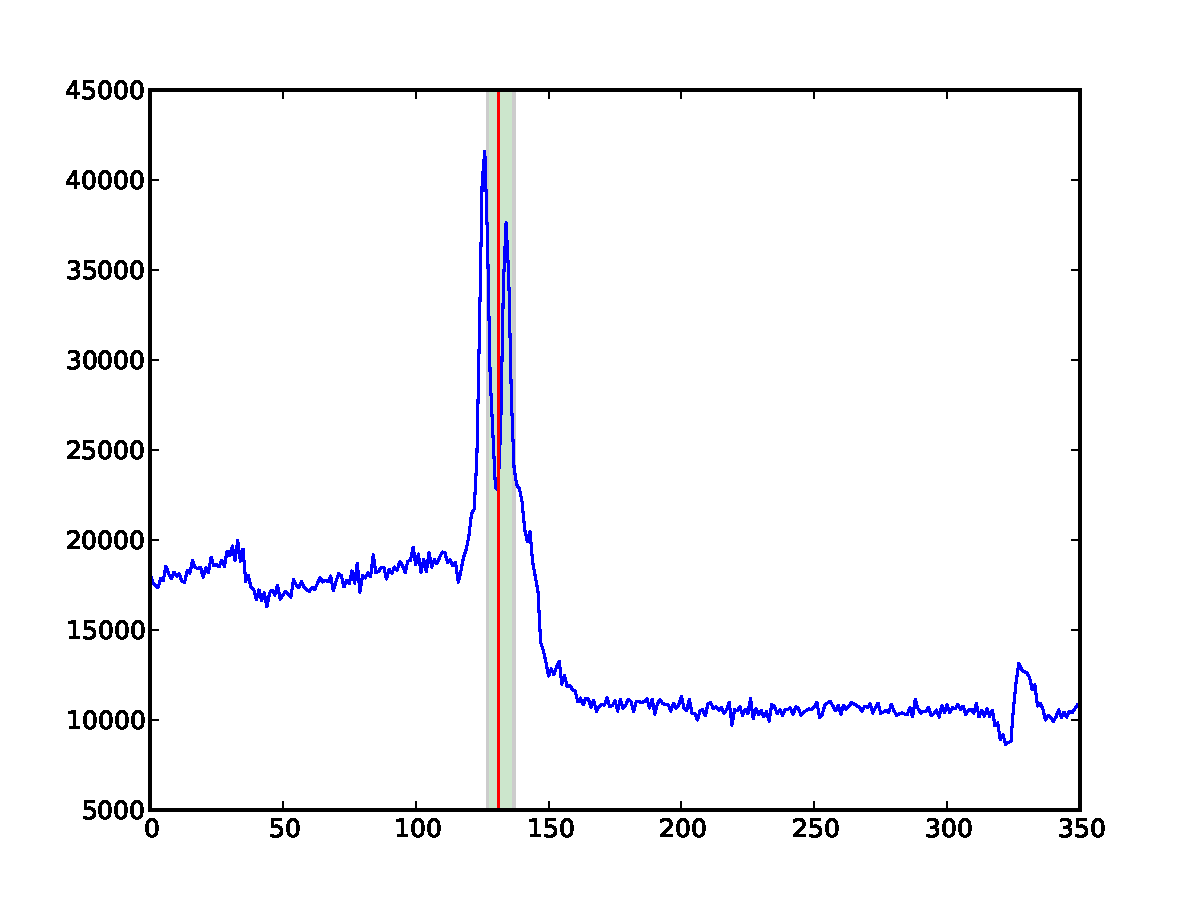
\includegraphics[width=\columnwidth]{figs/phcaxisprofile.pdf}%
		\caption{Brightness profile along the system axis for phase contrast image at Figure \ref{fig:pipetteaxis}. Green region corresponds to the user-supplied approximate pipette tip position. Red line denotes actual pipette tip position found. Other features are also clearly distinguishable.}%
		\label{fig:phcaxisprofile}%
		\end{figure}
		
		For phase contrast images (see Figure \ref{fig:phcaxisprofile}), the pipette tip ought to be a local minima or (in case of too small pipette and/or too bright illumination) a global maxima. Vesicle sides in turn are featured as steep jumps from dark to bright (so the inflection point is a choice for a feature position). 
		
		The pipette tip is first roughly located as the global maximum or minimum in the pipette tip search region, giving the position of the pipette tip with \emph{pixel resolution}. To get a \emph{subpixel resolution} of peak position its vicinity is fitted with some suitable profile (see Section \ref{subpix}) with parameters of the fit giving the value desired.
		
		As for inflection points, the rough positions are found by first applying a smoothing filter to the brightness profile, taking absolute value of smoothed profile's derivative (Savitzky-Golay \cite{Savitzky1964, Steinier1972} and Gauss smoothing/derivative filters are implemented for now) and than using user input for overestimated feature positions (see Section~\ref{getinput}) to define left and right search regions where global maxima for these regions are found, giving positions of steep jumps with \emph{pixel resolution} - see Figure \ref{fig:phcprofilegrad}. For \emph{subpixel resolution} the profile in the vicinity of estimated position must be fitted with suitable function with well-defined inflection point (see Section~\ref{subpix}).
		
		\begin{figure}%
		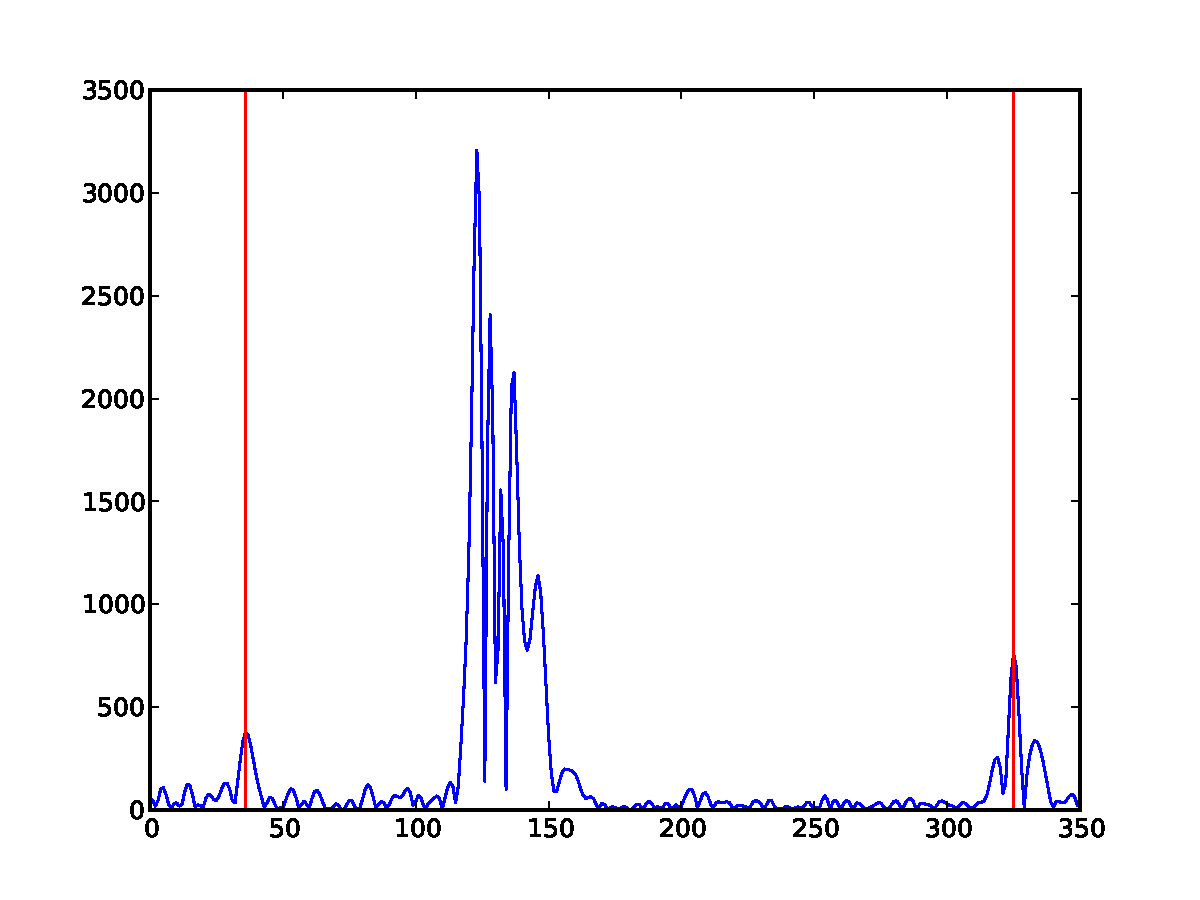
\includegraphics[width=\columnwidth]{figs/phcprofilegrad.pdf}%
		\caption{Result of applying gradient magnitude filter to gaussian-presmoothed profile from Figure \ref{fig:phcaxisprofile}. Red lines correspond to located features positions.}%
		\label{fig:phcprofilegrad}%
		\end{figure}
		
	\item \textbf{DIC images} \label{dicfeatures}
		
		For DIC images the aspirated tip is local minimum and the outer edge is local maximum in their respective search regions (or vice versa, depending on choice of polarizations) and pipette tip is (as with phase contrast images) either a local minimum or global maximum in the pipette tip search region. The fitting procedure by itself is the same as for peaks in~Section~\ref{phcfeatures}.
		
	\item \textbf{Subpixel resolution} \label{subpix}
		
		\emph{NOT YET IMPLEMENTED}
		
		Positions of features with subpixel resolutions can be found by making a non-linear least squares fit (\texttt{scipy.optimize.leastsq}, Levenberg-Marquardt implementation) of brightness profile in the vicinity of the pixel-resolved location of the feature using some suitable function. According to \cite{Bitler1999} brightness jumps on the edge of an object observed with phase contrast microscopy are described by integral sine function, with inflection point being the exact position of the object's edge. As for the peaks, for them the Gaussian bell function can be used with position of its maximum defining feature position with subpixel resolution.

\end{itemize}

\subsubsection{Calculation of derived parameters}\label{results}

\begin{figure}%
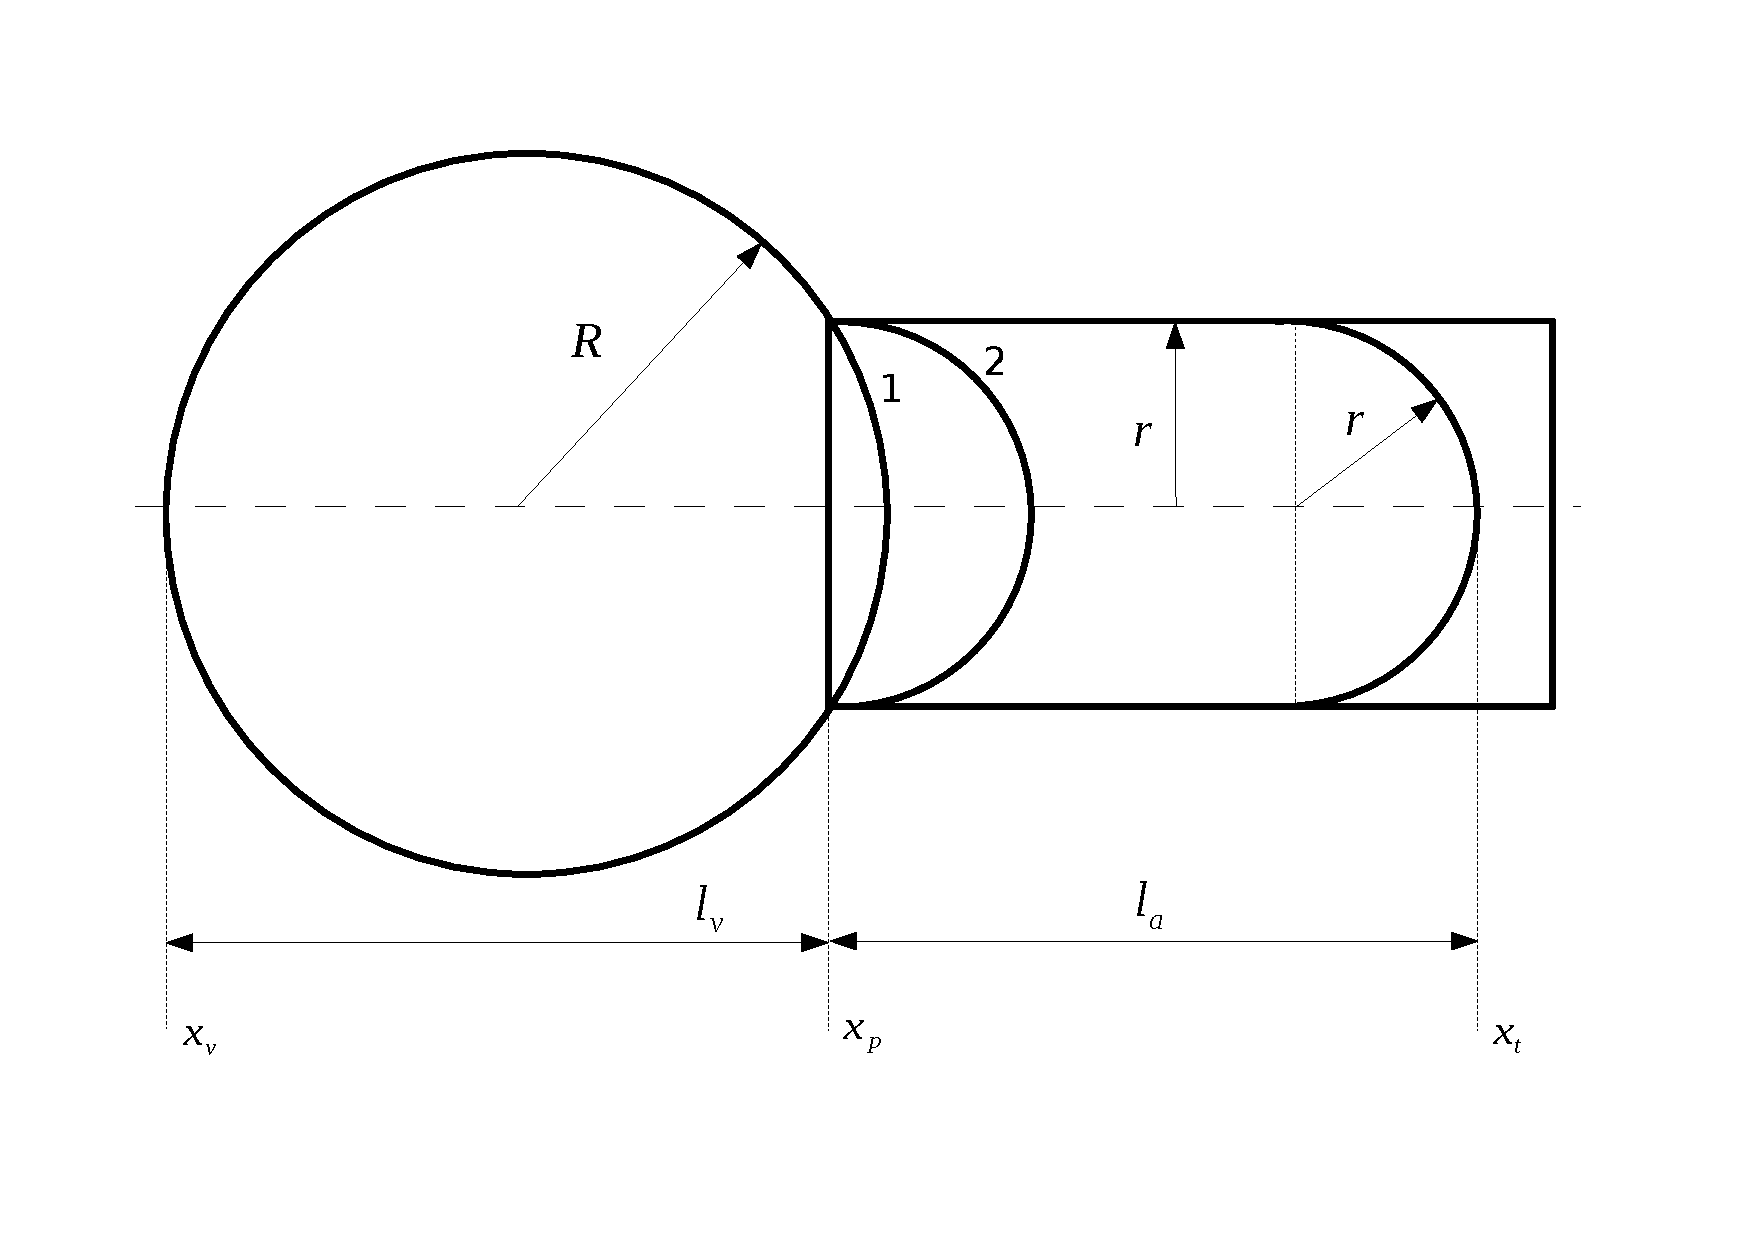
\includegraphics[width=\columnwidth]{figs/pipettesketch.pdf}%
\caption{Sketch of a vesicle aspirated into the pipette with explanation of parameters.\newline1: $l_a = 2R-l_v$.\newline2: $l_a = r$}%
\label{fig:pipettesketch}%
\end{figure}

Given positions of outer vesicle edge as $x_v$, pipette tip $x_p$ and aspirated vesicle tip $x_t$ plus the pipette radius $r$ together with their corresponding errors $\delta x_v$, $\delta x_p$, $\delta x_t$ and $\delta r$ and assuming total cylindrical symmetry of the system along the system axis and spherical form of the vesicle outside the pipette one can calculate the desired parameters (see Figure \ref{fig:pipettesketch}).

Denoting length of the vesicle part outside the pipette as $l_v = \left|x_p-x_v\right|$ with error $\delta l_v = \delta x_p + \delta x_v$ and the length of the aspirated tip as $l_a = \left|x_p-x_t\right|$ with error $\delta l_a = \delta x_p + \delta x_t$, the radius of the outside vesicle is
\begin{equation*}
R = \frac{{l_v}^2 + r^2}{2l_v}\;\;.
\end{equation*}
Corresponding error is then
\begin{equation*}
 \delta R = \sqrt{\frac{r^2}{{l_v}^2} \left(\delta r\right)^2 + \frac{1}{4}\left(1-\frac{r^2}{{l_v}^2}\right)^2 \left( \delta l_v\right) ^2}\;\;.
\end{equation*}
The surface of the inner part is
\begin{equation*}
S_\text{in} = \left\{
\begin{array}{ll}
	2\pi rl_a,& \text{if } l_a \geq r\\
	\pi\left({l_a}^2+r^2\right),&\text{if } 2R-l_v \leq l_a < r
\end{array}
\right.\;\;,
\end{equation*}
and its volume is
\begin{equation*}
V_{\text{in}} = \left\{
\begin{array}{ll}
	\pi r^2\left(l_a-\frac{r}{3}\right), & \text{if } l_a \geq r\\
	\frac{1}{6}\pi l_a\left(3r^2+{l_a}^2\right),&\text{if } 2R-l_v \leq l_a < r
\end{array}
\right.\;\;,
\end{equation*}
with errors
\begin{equation*}
 \delta S_\text{in} = \left\{
 \begin{array}{ll}
	2\pi \sqrt{{l_a}^2\left(\delta r\right)^2 + r^2\left(\delta l_a\right)^2},& \text{if } l_a \geq r\\
	2\pi \sqrt{{l_a}^2\left(\delta l_a\right)^2 + r^2\left(\delta r\right)^2},&\text{if } 2R-l_v \leq l_a < r
\end{array}
\right.\;\;
\end{equation*}
and
\begin{equation*}
\delta V_{\text{in}} = \left\{
\begin{array}{ll}
	\pi r \sqrt{r^2\left(\delta l_a\right)^2 + \left(2l_a-r\right)^2 \left(\delta r\right)^2}, & \text{if } l_a \geq r\\
	\frac{\pi}{2} \sqrt{4 r^2 {l_a}^2\left(\delta r\right)^2 + \left(r^2+{l_a}^2\right)^2 \left(\delta l_a\right)^2}, & \text{if } 2R-l_v \leq l_a < r
\end{array}
\right.\;\;.
\end{equation*}
The surface of the outer vesicle part is
\begin{equation*}
S_\text{out} = 2\pi Rl_v = \pi \left({l_v}^2+r^2\right)\;\;,
\end{equation*}
and it's volume is
\begin{equation*}
V_\text{out} = \frac{1}{6}\pi l_v\left(3r^2+{l_v}^2\right)\;\;
\end{equation*}
with errors
\begin{equation*}
\delta S_\text{out} = 2\pi\sqrt{{l_v}^2 \left(\delta l_v\right)^2 + r^2 \left( \delta r\right) ^2}\;\;
\end{equation*}
and
\begin{equation*}
\delta V_\text{out} = \frac{\pi}{2} \sqrt{4 r^2 {l_v}^2\left(\delta r\right)^2 + \left(r^2+{l_v}^2\right)^2 \left(\delta l_v\right)^2}\;\;.
\end{equation*}
Total area and volume of the vesicle are then $S = S_\text{out}+S_\text{in}$ and $V = V_\text{out}+V_\text{in}$ with errors $\delta S = \delta S_\text{out} + \delta S_\text{in}$ and $\delta V = \delta V_\text{out} + \delta V_\text{in}$ respectively.

\subsection{Data Analysis}\label{analysis}
\subsubsection{Classical procedure}
Having combined data acquired from image analysis together with corresponding pressure values obtained in experiment one finds elastic properties of membrane by fitting low-tension regime with logarithm and high-tension regime with linear functions. Also some corrections pointed out in \cite{Henriksen2004, Fournier2001} could be accounted for here, by trying to fit the whole range of pressures with one general function.

Currently tensions are calculated according to simple model after Evans:
\begin{equation}
\tau = \frac{P R_p}{2\left(1-\frac{R_p}{R_v}\right)}
\label{eq:tau-evans}
\end{equation}

Below is the list of currently implemented models/fittings.

Dilations:
\begin{itemize}
	\item simplest model $\alpha = \frac{S-S_0}{S_0}$
	\item corrected for initial aspiration after \cite{Henriksen2004}
	\begin{equation}
		\alpha = \left[
		 \frac{1}{2} \left(\frac{R_p}{R_{v0}}\right)^2 \frac{\Delta L}{R_p} 
		 + \left[1-\frac{3}{4}\left(\frac{R_p}{R_{v0}}\right)^3 \frac{\Delta L}{R_p} \right]^{\frac{2}{3}}
		 - 1 
		\right]\gamma
		\label{eq:alpha-henriksen}
	\end{equation}
	where $\displaystyle{\gamma = 1-\frac{2R_p L_0+R_p^2}{4R_{v0}^2}}$.
	\item approximated correction for initial aspiration after \cite{Henriksen2004} (made for testing)
	\begin{equation}
		\alpha = \frac{1}{2}\left[
		\left(\frac{R_p}{R_{v0}}\right)^2-\left(\frac{Rp}{R_{v0}}\right)^3\right]
		\frac{\Delta L}{R_p}\gamma
		\label{eq:alpha-henriksen-simple}
	\end{equation}
	where $\gamma$ as in equation \ref{eq:alpha-henriksen}.
\end{itemize}

Fittings (done with Orthogonal Distance Regression):
\begin{itemize}
	\item Simple model for bending rigidity: $\alpha=\frac{1}{8\pi\kappa}\ln{\frac{\tau}{\tau_0}}$
	\item Simple model for stretching elasticity: $\alpha=\frac{\tau}{K}+\alpha_0$
\end{itemize}

\subsubsection{Modern procedure}
The overall ultimate goal is to implement a MCMC (Markov Chain Monte Carlo) algorithm found in  \cite{Henriksen2004}.